% Lecture 10: exact content reconstruction of source slides 1--50 from
% Lecture9/Linear algebra_ 06_4.pptx. No source slide is embedded as an image.
% Compile from the repository root with:
%   pdflatex -interaction=nonstopmode -halt-on-error -output-directory=Lecture10 Lecture10/lecture10.tex
\pdfminorversion=7
\documentclass[aspectratio=169]{beamer}

\usepackage{amsmath,amssymb,mathtools}
\usepackage{array,booktabs,multirow}
\usepackage{xcolor}
\usepackage{tikz}
\usepackage{iftex}
\ifPDFTeX
  \usepackage[UTF8,heading=false]{ctex}
\else
  \usepackage{fontspec}
  \usepackage{xeCJK}
  \setCJKmainfont{Microsoft YaHei}
\fi
\usetikzlibrary{arrows.meta,calc,positioning}

\makeatletter
\def\input@path{{./}{../}{Lecture10/}}
\makeatother

\mode<presentation>{
  \usetheme{OSUCSE169}
  \setbeamercovered{invisible}
}
\setbeamertemplate{navigation symbols}{}
\setbeamertemplate{footline}[frame number]
\setbeamercolor{headline}{fg=black,bg=black}
\setbeamercolor{section in head/foot}{bg=gray}
\setbeamertemplate{headline}{%
  \begin{beamercolorbox}[ht=2.25ex,dp=3.75ex]{section in head/foot}
    \insertnavigation{\paperwidth}
  \end{beamercolorbox}}

\definecolor{lecturegreen}{RGB}{48,105,21}
\definecolor{sourcecyan}{RGB}{0,132,166}
\definecolor{sourceblue}{RGB}{0,112,192}

\newcommand{\R}{\mathbb{R}}
\newcommand{\vect}[1]{\mathbf{#1}}
\newcommand{\Span}{\operatorname{Span}}
\newcommand{\Col}{\operatorname{Col}}
\newcommand{\Nul}{\operatorname{Nul}}
\newcommand{\sourcehead}[1]{\textcolor{sourcecyan}{\textbf{#1}}}
\newcommand{\chaptercard}[4]{%
  \begin{frame}[plain]
    \vfill
    {\Huge\color{lecturegreen}\bfseries #1}\hspace{1.2em}%
    {\Huge\color{sourcecyan} #2}
    \vspace{2.4cm}

    {\Huge\color{sourcecyan}\bfseries #3}\par\medskip
    {\LARGE\color{sourcecyan}\bfseries #4}
    \vfill
  \end{frame}}

\begin{document}
% Source slide 1
\section[4.1 Vector Spaces]{4.1 Vector Spaces and Subspaces}
\chaptercard{4}{Vector Spaces}{4.1}{VECTOR SPACES AND SUBSPACES}

% Source slide 2
\begin{frame}{Overview of Linear Algebra}
\centering
\Large
\begin{align*}
\text{平面（2维）解析几何} &\Longleftrightarrow \R^2\text{的线性代数},\\
\text{空间（3维）解析几何} &\Longleftrightarrow \R^3\text{的线性代数},\\
\text{$n$维数组空间解析几何} &\Longleftrightarrow \R^n\text{的线性代数}.
\end{align*}
\vspace{0.4cm}
\begin{tikzpicture}[>=Stealth,thick]
  \node[draw,fill=yellow,minimum width=4.8cm,minimum height=1.0cm] (v) {一般的向量空间};
  \node[right=5.5cm of v] (m) {矩阵的运算};
  \draw[<->,line width=2pt,draw=pink!60!black] ($(v.north)+(0,0.2)$) -- node[right,black]{\Large\itshape Basis} ++(0,1.8);
  \draw[<->,line width=2pt,draw=pink!60!black] ($(m.north)+(0,0.2)$) -- ++(0,1.8);
\end{tikzpicture}
\end{frame}

% Source slide 3
\begin{frame}[shrink=11]{VECTOR SPACES AND SUBSPACES}
\begin{itemize}
\item \textbf{Definition:} A \textcolor{blue!60}{\textbf{vector space}} is a nonempty set $V$ of objects, called \emph{vectors}, on which are defined two operations, called \emph{addition and multiplication by scalars} (real numbers), subject to the ten axioms (or rules) listed below. The axioms must hold for all vectors $\vect u$, $\vect v$, and $\vect w$ in $V$ and for all scalars $c$ and $d$.
\end{itemize}
\begin{enumerate}
\item The sum of $\vect u$ and $\vect v$, denoted by $\vect u+\vect v$, is in $V$.
\item $\vect u+\vect v=\vect v+\vect u$.
\item $(\vect u+\vect v)+\vect w=\vect u+(\vect v+\vect w)$.
\item There is a zero vector $0$ in $V$ such that
\[
\vect u+0=\vect u.
\]
\end{enumerate}
\end{frame}

% Source slide 4
\begin{frame}[shrink=9]{VECTOR SPACES AND SUBSPACES}
\begin{enumerate}
\setcounter{enumi}{4}
\item For each $\vect u$ in $V$, there is a vector $-\vect u$ in $V$ such that $\vect u+(-\vect u)=0$.
\item The scalar multiple of $\vect u$ by $c$, denoted by $c\vect u$, is in $V$.
\item $c(\vect u+\vect v)=c\vect u+c\vect v$.
\item $(c+d)\vect u=c\vect u+d\vect u$.
\item $c(d\vect u)=(cd)\vect u$.
\item $1\vect u=\vect u$.
\end{enumerate}
\begin{itemize}
\item Using these axioms, we can show that \textcolor{red}{the zero vector in Axiom 4 is unique}, and the vector $-\vect u$, called the \textbf{negative} of $\vect u$, in Axiom 5 is unique for each $\vect u$ in $V$.
\end{itemize}
\end{frame}

% Source slide 5
\begin{frame}[shrink=8]{VECTOR SPACES AND SUBSPACES}
\begin{itemize}
\item For each $\vect u$ in $V$ and scalar $c$,
\end{itemize}
\begin{align}
0\vect u&=0 \tag{1}\\
c0&=0 \tag{2}\\
-\vect u&=(-1)\vect u. \tag{3}
\end{align}
\vspace{0.6cm}
{\Large\color{sourcecyan}Examples --- Vector Spaces of Real Number Vectors}
\medskip

\textcolor{red!70!black}{\textbf{EXAMPLE 1}}\quad
The spaces $\R^n$, where $n\geq1$, are the premier examples of vector spaces. The geometric intuition developed for $\R^3$ will help you understand and visualize many concepts throughout the chapter.
\end{frame}

% Source slide 6
\begin{frame}[shrink=12]{Examples --- Vector Spaces of Arrows}
\begin{itemize}
\item \textbf{Example 2:} Let $V$ be the set of all arrows (directed line segments) in three-dimensional space, with two arrows regarded as equal if they have the same length and point in the same direction. Define addition by the parallelogram rule, and for each $\vect v$ in $V$, define $c\vect v$ to be the arrow whose length is $c$ times the length of $\vect v$, pointing in the same direction as $\vect v$ if $c\geq0$ and otherwise pointing in the opposite direction.
\item See the following figure below. Show that $V$ is a vector space.
\end{itemize}
\centering
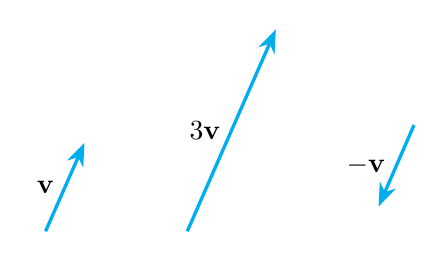
\begin{tikzpicture}[>=Stealth,scale=0.9]
  \draw[->,very thick,cyan] (0,0)--(0.55,1.25) node[midway,left,black] {$\vect v$};
  \draw[->,very thick,cyan] (2,0)--(3.25,2.85) node[midway,left,black] {$3\vect v$};
  \draw[->,very thick,cyan] (5.2,1.5)--(4.7,0.35) node[midway,left,black] {$-\vect v$};
\end{tikzpicture}
\end{frame}

% Source slide 7
\begin{frame}[shrink=13]
\begin{itemize}
\item \textbf{Solution:} The definition of $V$ is geometric, using concepts of length and direction.
\item No $x\ y\ z$-coordinate system is involved.
\item An arrow of zero length is a single point and represents the zero vector.
\item The negative of $\vect v$ is $-\vect v$.
\item So Axioms 1, 4, 5, 6, and 10 are evident. See the figures on the next slide.
\end{itemize}
\begin{columns}[T]
\column{.48\textwidth}
\centering
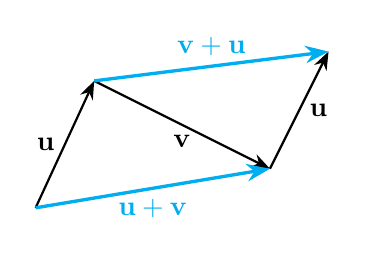
\begin{tikzpicture}[>=Stealth,scale=0.62]
  \coordinate (A) at (0,0); \coordinate (B) at (1.2,2.6); \coordinate (C) at (6.0,3.2); \coordinate (D) at (4.8,0.8);
  \draw[->,thick] (A)--(B) node[midway,left] {$\vect u$};
  \draw[->,thick] (D)--(C) node[midway,right] {$\vect u$};
  \draw[->,thick] (B)--(D) node[midway,below] {$\vect v$};
  \draw[->,very thick,cyan] (A)--(D) node[midway,below] {$\vect u+\vect v$};
  \draw[->,very thick,cyan] (B)--(C) node[midway,above] {$\vect v+\vect u$};
\end{tikzpicture}

$\vect u+\vect v=\vect v+\vect u$.
\column{.48\textwidth}
\centering
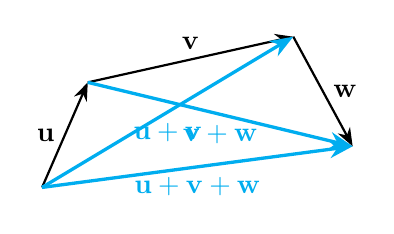
\begin{tikzpicture}[>=Stealth,scale=0.58]
  \coordinate (A) at (0,0); \coordinate (B) at (1.0,2.3); \coordinate (C) at (5.5,3.3); \coordinate (D) at (6.8,0.9);
  \draw[->,thick] (A)--(B) node[midway,left] {$\vect u$};
  \draw[->,thick] (B)--(C) node[midway,above] {$\vect v$};
  \draw[->,thick] (C)--(D) node[midway,right] {$\vect w$};
  \draw[->,very thick,cyan] (A)--(C) node[midway,below] {$\vect u+\vect v$};
  \draw[->,very thick,cyan] (B)--(D) node[midway,below] {$\vect v+\vect w$};
  \draw[->,very thick,cyan] (A)--(D) node[midway,below] {$\vect u+\vect v+\vect w$};
\end{tikzpicture}

$(\vect u+\vect v)+\vect w=\vect u+(\vect v+\vect w)$.
\end{columns}
\end{frame}

% Source slide 8
\begin{frame}[shrink=24]{Examples --- Vector Spaces of Functions}
\textcolor{red!70!black}{\textbf{EXAMPLE 5}}\quad
Let $V$ be the set of all real-valued functions defined on a set $\mathbb D$. (Typically, $\mathbb D$ is the set of real numbers or some interval on the real line.) Functions are added in the usual way: $\vect f+\vect g$ is the function whose value at $t$ in the domain $\mathbb D$ is $f(t)+g(t)$. Likewise, for a scalar $c$ and an $\vect f$ in $V$, the scalar multiple $c\vect f$ is the function whose value at $t$ is $cf(t)$. For instance, if $\mathbb D=\R$, $f(t)=1+\sin 2t$, and $g(t)=2+.5t$, then
\[
(\vect f+\vect g)(t)=3+\sin 2t+.5t
\qquad\text{and}\qquad
(2\vect g)(t)=4+t.
\]
Two functions in $V$ are equal if and only if their values are equal for every $t$ in $\mathbb D$. Hence the zero vector in $V$ is the function that is identically zero, $f(t)=0$ for all $t$, and the negative of $\vect f$ is $(-1)\vect f$. Axioms 1 and 6 are obviously true, and the other axioms follow from properties of the real numbers, so $V$ is a vector space.

\begin{center}
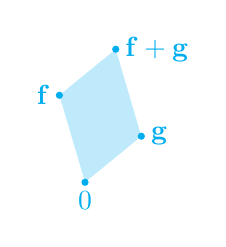
\begin{tikzpicture}[>=Stealth,scale=0.65]
  \coordinate (O) at (0,0); \coordinate (F) at (-0.5,1.7); \coordinate (G) at (1.1,0.9); \coordinate (S) at (0.6,2.6);
  \fill[cyan!25] (O)--(F)--(S)--(G)--cycle;
  \fill[cyan] (O) circle (2pt) node[below] {$0$};
  \fill[cyan] (F) circle (2pt) node[left] {$\vect f$};
  \fill[cyan] (G) circle (2pt) node[right] {$\vect g$};
  \fill[cyan] (S) circle (2pt) node[right] {$\vect f+\vect g$};
\end{tikzpicture}

\textbf{FIGURE 5}\quad The sum of two vectors (functions).
\end{center}
\end{frame}

% Source slide 9
\begin{frame}[shrink=9]{SUBSPACES}
\begin{itemize}
\item \textbf{Definition:} A \textbf{subspace} of a vector space $V$ is a subset $H$ of $V$ that has three properties:
\end{itemize}
\begin{enumerate}
\item[(a.)] The zero vector of $V$ is in $H$.
\item[(b.)] $H$ is closed under vector addition. That is, for each $\vect u$ and $\vect v$ in $H$, the sum $\vect u+\vect v$ is in $H$.
\item[(c.)] $H$ is closed under multiplication by scalars. That is, for each $\vect u$ in $H$ and each scalar $c$, the vector $c\vect u$ is in $H$.
\end{enumerate}
\end{frame}

% Source slide 10
\begin{frame}{SUBSPACES}
\begin{itemize}
\item Properties (a), (b), and (c) guarantee that a subspace $H$ of $V$ is itself a \emph{vector space}, under the vector space operations already defined in $V$.
\item Every subspace is a vector space.
\item Conversely, every \emph{vector space} is a subspace (of itself and possibly of other larger spaces).
\end{itemize}
\end{frame}

% Source slide 11
\begin{frame}[shrink=10]
\textcolor{red!70!black}{\textbf{EXAMPLE 6}}\quad
The set consisting of only the zero vector in a vector space $V$ is a subspace of $V$, called the \textbf{zero subspace} and written as $\{0\}$.
\vspace{0.5cm}
\begin{columns}[T]
\column{.48\textwidth}
\centering
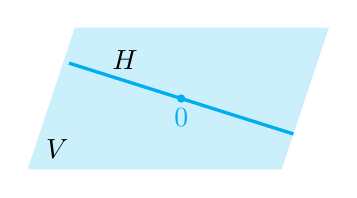
\begin{tikzpicture}[scale=0.75]
  \fill[cyan!20] (0,0)--(4.3,0)--(5.1,2.4)--(0.8,2.4)--cycle;
  \draw[cyan,very thick] (0.7,1.8)--(4.5,0.6) node[pos=.25,above,black] {$H$};
  \fill[cyan] (2.6,1.2) circle (2pt) node[below] {$0$};
  \node at (.5,.35) {$V$};
\end{tikzpicture}

\textbf{FIGURE 6}\par A subspace of $V$.
\column{.48\textwidth}
\centering
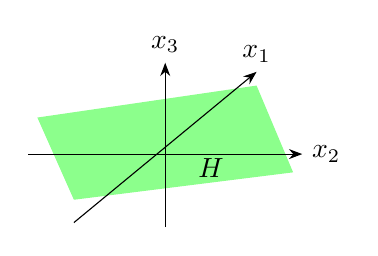
\begin{tikzpicture}[>=Stealth,scale=0.58]
  \fill[green!45] (-2,-1)--(2.8,-.4)--(2,1.5)--(-2.8,.8)--cycle;
  \draw[->] (-3,0)--(3,0) node[right] {$x_2$};
  \draw[->] (-2,-1.5)--(2,1.8) node[above] {$x_1$};
  \draw[->] (0,-1.6)--(0,2) node[above] {$x_3$};
  \node at (1,-.3) {$H$};
\end{tikzpicture}

\textbf{FIGURE 7}\par The $x_1x_2$-plane as a subspace of $\R^3$.
\end{columns}
\end{frame}

% Source slide 12
\begin{frame}[shrink=11]
\textcolor{red!70!black}{\textbf{EXAMPLE 9}}\quad
A plane in $\R^3$ \emph{not} through the origin is not a subspace of $\R^3$, because the plane does not contain the zero vector of $\R^3$. Similarly, a line in $\R^2$ \emph{not} through the origin, such as in Figure 8, is not a subspace of $\R^2$.
\vspace{0.7cm}
\begin{center}
\begin{tikzpicture}[>=Stealth,scale=0.8]
  \draw[->] (-2.2,0)--(2.4,0) node[right] {$x_1$};
  \draw[->] (0,-1.2)--(0,2.2) node[above] {$x_2$};
  \draw[cyan,very thick] (-1.5,1.4)--(1.8,-.7) node[midway,above] {$H$};
\end{tikzpicture}

\textbf{FIGURE 8}\par A line that is not a vector space.
\end{center}
\end{frame}

% Source slide 13
\begin{frame}{A SUBSPACE SPANNED BY A SET}
\begin{itemize}
\item ------ \textcolor{cyan}{\emph{the most common ways of describing a subspace}}
\item As the term \textcolor{sourceblue}{\textbf{linear combination}} refers to any sum of scalar multiples of vectors, and \textcolor{sourceblue}{\textbf{$\Span\{\vect v_1,\ldots,\vect v_p\}$}} denotes the set of all vectors that can be written as linear combinations of $\vect v_1,\ldots,\vect v_p$.
\end{itemize}
\end{frame}

% Source slide 14
\begin{frame}[shrink=14]{A SUBSPACE SPANNED BY A SET}
\begin{itemize}
\item \textbf{Example 10:} Given $\vect v_1$ and $\vect v_2$ in a vector space $V$, let $H=\Span\{\vect v_1,\vect v_2\}$. Show that $H$ is a subspace of $V$.
\item \textbf{Solution:} The zero vector is in $H$, since $0=0\vect v_1+0\vect v_2$.
\item To show that $H$ is closed under vector addition, take two arbitrary vectors in $H$, say,
\[
\vect u=s_1\vect v_1+s_2\vect v_2
\qquad\text{and}\qquad
\vect w=t_1\vect v_1+t_2\vect v_2.
\]
\item By Axioms 2, 3, and 8 for the vector space $V$,
\begin{align*}
\vect u+\vect w&=(s_1\vect v_1+s_2\vect v_2)+(t_1\vect v_1+t_2\vect v_2)\\
&=(s_1+t_1)\vect v_1+(s_2+t_2)\vect v_2.
\end{align*}
\end{itemize}
\end{frame}

% Source slide 15
\begin{frame}[shrink=13]{A SUBSPACE SPANNED BY A SET}
\begin{itemize}
\item So $\vect u+\vect w$ is in $H$.
\item Furthermore, if $c$ is any scalar, then by Axioms 7 and 9,
\[
c\vect u=c(s_1\vect v_1+s_2\vect v_2)=(cs_1)\vect v_1+(cs_2)\vect v_2,
\]
which shows that $c\vect u$ is in $H$ and $H$ is closed under scalar multiplication.
\item Thus $H$ is a subspace of $V$.
\end{itemize}
\begin{flushright}
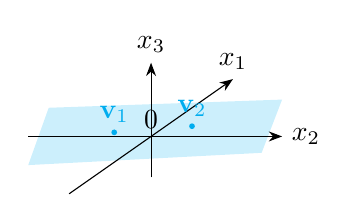
\begin{tikzpicture}[>=Stealth,scale=0.52]
  \fill[cyan!20] (-3,-.7)--(2.7,-.4)--(3.2,.9)--(-2.5,.7)--cycle;
  \draw[->] (-3,0)--(3.2,0) node[right] {$x_2$};
  \draw[->] (-2,-1.4)--(2,1.4) node[above] {$x_1$};
  \draw[->] (0,-1)--(0,1.8) node[above] {$x_3$};
  \fill[cyan] (-.9,.1) circle (2pt) node[above] {$\vect v_1$};
  \fill[cyan] (1,.25) circle (2pt) node[above] {$\vect v_2$};
  \node at (0,.4) {$0$};
\end{tikzpicture}

\textbf{FIGURE 9}\quad An example of a subspace.
\end{flushright}
\end{frame}

% Source slide 16
\begin{frame}[shrink=9]{A SUBSPACE SPANNED BY A SET}
\begin{itemize}
\item \sourcehead{Theorem 1:} If $\vect v_1,\ldots,\vect v_p$ are in a vector space $V$, then $\Span\{\vect v_1,\ldots,\vect v_p\}$ is a subspace of $V$.
\item We call $\Span\{\vect v_1,\ldots,\vect v_p\}$ \textbf{the subspace spanned} (or \textbf{generated}) by $\{\vect v_1,\ldots,\vect v_p\}$.
\item Give any subspace $H$ of $V$, a \textbf{spanning} (or \textbf{generating}) set for $H$ is a set $\{\vect v_1,\ldots,\vect v_p\}$ in $H$ such that
\[
H=\Span\{\vect v_1,\ldots,\vect v_p\}.
\]
\end{itemize}
\end{frame}

% Source slide 17
\begin{frame}[shrink=18]
\textcolor{red!70!black}{\textbf{EXAMPLE 11}}\quad
Let $H$ be the set of all vectors of the form $(a-3b,b-a,a,b)$, where $a$ and $b$ are arbitrary scalars. That is, let
\[
H=\{(a-3b,b-a,a,b):a\text{ and }b\text{ in }\R\}.
\]
Show that $H$ is a subspace of $\R^4$.

\textcolor{red!70!black}{\textbf{SOLUTION}}\quad Write the vectors in $H$ as column vectors. Then an arbitrary vector in $H$ has the form
\[
\begin{bmatrix}a-3b\\b-a\\a\\b\end{bmatrix}
=a\underbrace{\begin{bmatrix}1\\-1\\1\\0\end{bmatrix}}_{\vect v_1}
+b\underbrace{\begin{bmatrix}-3\\1\\0\\1\end{bmatrix}}_{\vect v_2}.
\]
This calculation shows that $H=\Span\{\vect v_1,\vect v_2\}$, where $\vect v_1$ and $\vect v_2$ are the vectors indicated above. Thus $H$ is a subspace of $\R^4$ by Theorem 1.

\begin{center}
Calculations with the infinitely many vectors in $H$\\[-.2ex]
$\Updownarrow$\\[-.2ex]
Operations with the finite number of vectors in the spanning set.
\end{center}
\end{frame}

% Source slide 18
\section[4.2 Null and Column Spaces]{4.2 Null Spaces, Column Spaces, and Linear Transformations}
\chaptercard{4}{Vector Spaces}{4.2}{NULL SPACES, COLUMN SPACES, AND LINEAR TRANSFORMATIONS}

% Source slide 19
\begin{frame}[shrink=15]{NULL SPACE OF A MATRIX}
\begin{itemize}
\item \textbf{Definition:} The \textcolor{sourceblue}{\textbf{null space}} of an $m\times n$ matrix $A$, written as $\Nul A$, is the set of all solutions of the homogeneous equation $A\vect x=0$. In set notation,
\[
\Nul A=\{\vect x:\vect x\text{ is in }\R^n\text{ and }A\vect x=0\}.
\]
\item \sourcehead{Theorem 2:} The null space of an $m\times n$ matrix $A$ is a subspace of $\R^n$. Equivalently, the set of all solutions to a system $A\vect x=0$ of $m$ homogeneous linear equations in $n$ unknowns is a subspace of $\R^n$.
\item \textbf{Proof:} $\Nul A$ is a subset of $\R^n$ because $A$ has $n$ columns.
\item We need to show that $\Nul A$ satisfies the three properties of a subspace.
\end{itemize}
\end{frame}

% Source slide 20
\begin{frame}[shrink=13]{NULL SPACE OF A MATRIX}
\begin{itemize}
\item $0$ is in $\Nul A$.
\item Next, let $\vect u$ and $\vect v$ represent any two vectors in $\Nul A$.
\item Then
\[
A\vect u=0\qquad\text{and}\qquad A\vect v=0.
\]
\item To show that $\vect u+\vect v$ is in $\Nul A$, we must show that $A(\vect u+\vect v)=0$.
\item Using a property of matrix multiplication, compute
\[
A(\vect u+\vect v)=A\vect u+A\vect v=0+0=0.
\]
\item Thus $\vect u+\vect v$ is in $\Nul A$, and $\Nul A$ is closed under vector addition.
\end{itemize}
\end{frame}

% Source slide 21
\begin{frame}[shrink=10]{NULL SPACE OF A MATRIX}
\begin{itemize}
\item Finally, if $c$ is any scalar, then
\[
A(c\vect u)=c(A\vect u)=c(0)=0,
\]
which shows that $c\vect u$ is in $\Nul A$.
\item Thus $\Nul A$ is a subspace of $\R^n$.
\item \textbf{An Explicit Description of $\Nul A$}
\item There is no obvious relation between vectors in $\Nul A$ and the entries in $A$.
\item We say that $\Nul A$ is defined \emph{implicitly}, because it is defined by a condition that must be checked.
\end{itemize}
\end{frame}

% Source slide 22
\begin{frame}[shrink=10]{NULL SPACE OF A MATRIX}
\begin{itemize}
\item No explicit list or description of the elements in $\Nul A$ is given.
\item \emph{Solving} the equation $A\vect x=0$ amounts to producing an \emph{explicit} description of $\Nul A$.
\item \textbf{Example 3:} Find a spanning set for the null space of the matrix
\[
A=\begin{bmatrix}
-3&6&-1&1&-7\\
1&-2&2&3&-1\\
2&-4&5&8&-4
\end{bmatrix}.
\]
\end{itemize}
\end{frame}

% Source slide 23
\begin{frame}[shrink=15]{NULL SPACE OF A MATRIX}
\begin{itemize}
\item \textbf{Solution:} The first step is to find the general solution of $A\vect x=0$ in terms of free variables.
\item Row reduce the augmented matrix $[A\ \ 0]$ to reduce echelon form in order to write the basic variables in terms of the free variables:
\end{itemize}
\[
\begin{bmatrix}
1&-2&0&-1&3&0\\
0&0&1&2&-2&0\\
0&0&0&0&0&0
\end{bmatrix},
\qquad
\begin{aligned}
x_1-2x_2-x_4+3x_5&=0,\\
x_3+2x_4-2x_5&=0,\\
0&=0.
\end{aligned}
\]
\end{frame}

% Source slide 24
\begin{frame}[shrink=18]{NULL SPACE OF A MATRIX}
\begin{itemize}
\item The general solution is $x_1=2x_2+x_4-3x_5$, $x_3=-2x_4+2x_5$, with $x_2,x_4$, and $x_5$ free.
\item Next, decompose the vector giving the general solution into a linear combination of \emph{vectors where the weights are the free variables}. That is,
\end{itemize}
\[
\begin{bmatrix}x_1\\x_2\\x_3\\x_4\\x_5\end{bmatrix}
=\begin{bmatrix}2x_2+x_4-3x_5\\x_2\\-2x_4+2x_5\\x_4\\x_5\end{bmatrix}
=x_2\underbrace{\begin{bmatrix}2\\1\\0\\0\\0\end{bmatrix}}_{\vect u}
+x_4\underbrace{\begin{bmatrix}1\\0\\-2\\1\\0\end{bmatrix}}_{\vect v}
+x_5\underbrace{\begin{bmatrix}-3\\0\\2\\0\\1\end{bmatrix}}_{\vect w}.
\]
\end{frame}

% Source slide 25
\begin{frame}[shrink=15]{NULL SPACE OF A MATRIX}
\[
=x_2\vect u+x_4\vect v+x_5\vect w \tag{3}
\]
\begin{itemize}
\item Every linear combination of $\vect u$, $\vect v$, and $\vect w$ is an element of $\Nul A$.
\item Thus $\{\vect u,\vect v,\vect w\}$ is a spanning set for $\Nul A$.
\end{itemize}
\begin{enumerate}
\item The spanning set produced by the method in Example (3) is automatically linearly independent because the free variables are the weights on the spanning vectors.
\item When $\Nul A$ contains nonzero vectors, the number of vectors in the spanning set for $\Nul A$ equals the number of free variables in the equation $A\vect x=0$.
\end{enumerate}
\end{frame}

% Source slide 26
\begin{frame}[shrink=13]{COLUMN SPACE OF A MATRIX}
\begin{itemize}
\item \textbf{Definition:} The column space of an $m\times n$ matrix $A$, written as $\Col A$, is the set of all linear combinations of the columns of $A$. If $A=[\vect a_1\ \cdots\ \vect a_n]$, then
\[
\Col A=\Span\{\vect a_1,\ldots,\vect a_n\}.
\]
\item \sourcehead{Theorem 3:} The column space of an $m\times n$ matrix $A$ is a subspace of $\R^m$.
\item A typical vector in $\Col A$ can be written as $A\vect x$ for some $\vect x$ because the notation $A\vect x$ stands for a linear combination of the columns of $A$. That is,
\[
\Col A=\{\vect b:\vect b=A\vect x\text{ for some }\vect x\text{ in }\R^n\}.
\]
\end{itemize}
\end{frame}

% Source slide 27
\begin{frame}[shrink=13]{COLUMN SPACE OF A MATRIX}
\begin{itemize}
\item The column space of an $m\times n$ matrix $A$ is all of $\R^m$ if and only if the equation $A\vect x=\vect b$ has a solution for each $\vect b$ in $\R^m$.
\item \textbf{Example 7:} Let
\[
A=\begin{bmatrix}2&4&-2&1\\-2&-5&7&3\\3&7&-8&6\end{bmatrix},
\qquad
\vect u=\begin{bmatrix}3\\-2\\-1\\0\end{bmatrix},
\qquad
\vect v=\begin{bmatrix}3\\-1\\3\end{bmatrix}.
\]
\end{itemize}
\end{frame}

% Source slide 28
\begin{frame}[shrink=14]{COLUMN SPACE OF A MATRIX}
\begin{enumerate}
\item[(a.)] Determine if $\vect u$ is in $\Nul A$. Could $\vect u$ be in $\Col A$?
\item[(b.)] Determine if $\vect v$ is in $\Col A$. Could $\vect v$ be in $\Nul A$?
\end{enumerate}
\begin{itemize}
\item \textbf{Solution:}
\end{itemize}
\begin{enumerate}
\item[(a.)] An explicit description of $\Nul A$ is not needed here. Simply compute the product $A\vect u$.
\end{enumerate}
\[
A\vect u=
\begin{bmatrix}2&4&-2&1\\-2&-5&7&3\\3&7&-8&6\end{bmatrix}
\begin{bmatrix}3\\-2\\-1\\0\end{bmatrix}
=\begin{bmatrix}0\\-3\\3\end{bmatrix}
\ne\begin{bmatrix}0\\0\\0\end{bmatrix}.
\]
\end{frame}

% Source slide 29
\begin{frame}[shrink=14]{COLUMN SPACE OF A MATRIX}
\begin{itemize}
\item $\vect u$ is \emph{not} a solution of $A\vect x=0$, so $\vect u$ is not in $\Nul A$.
\item Also, with four entries, $\vect u$ could not possibly be in $\Col A$, since $\Col A$ is a subspace of $\R^3$.
\end{itemize}
\begin{enumerate}
\item[(b.)] Reduce $[A\ \ \vect v]$ to an echelon form.
\end{enumerate}
\[
[A\ \ \vect v]=
\begin{bmatrix}2&4&-2&1&3\\-2&-5&7&3&-1\\3&7&-8&6&3\end{bmatrix}
\sim
\begin{bmatrix}2&4&-2&1&3\\0&1&-5&-4&-2\\0&0&0&17&1\end{bmatrix}.
\]
\begin{itemize}
\item The equation $A\vect x=\vect v$ is consistent, so $\vect v$ is in $\Col A$.
\end{itemize}
\end{frame}

% Source slide 30
\begin{frame}[shrink=13]{CONTRAST BETWEEN $\Nul A$ AND $\Col A$ FOR AN $m\times n$ MATRIX $A$}
\renewcommand{\arraystretch}{1.35}
\begin{tabular}{|>{\raggedright\arraybackslash}p{.45\linewidth}|>{\raggedright\arraybackslash}p{.45\linewidth}|}
\hline
\centering $\Nul A$ & \centering $\Col A$\tabularnewline
\hline
1. $\Nul A$ is a subspace of $\R^n$. & 1. $\Col A$ is a subspace of $\R^m$.\\
\hline
2. $\Nul A$ is implicitly defined; \emph{i.e.}, you are given only a condition $(A\vect x=0)$ that vectors in $\Nul A$ must satisfy. & 2. $\Col A$ is explicitly defined; \emph{i.e.}, you are told how to build vectors in $\Col A$.\\
\hline
\end{tabular}
\end{frame}

% Source slide 31
\begin{frame}[shrink=13]{CONTRAST BETWEEN $\Nul A$ AND $\Col A$ FOR AN $m\times n$ MATRIX $A$}
\renewcommand{\arraystretch}{1.35}
\begin{tabular}{|>{\raggedright\arraybackslash}p{.45\linewidth}|>{\raggedright\arraybackslash}p{.45\linewidth}|}
\hline
3. It takes time to find vectors in $\Nul A$. Row operations on $[A\ \ 0]$ are required. & 3. It is easy to find vectors in $\Col A$. The columns of a are displayed; others are formed from them.\\
\hline
4. There is no obvious relation between $\Nul A$ and the entries in $A$. & 4. There is an obvious relation between $\Col A$ and the entries in $A$, since each column of $A$ is in $\Col A$.\\
\hline
\end{tabular}
\end{frame}

% Source slide 32
\begin{frame}[shrink=13]{CONTRAST BETWEEN $\Nul A$ AND $\Col A$ FOR AN $m\times n$ MATRIX $A$}
\renewcommand{\arraystretch}{1.35}
\begin{tabular}{|>{\raggedright\arraybackslash}p{.45\linewidth}|>{\raggedright\arraybackslash}p{.45\linewidth}|}
\hline
5. A typical vector $\vect v$ in $\Nul A$ has the property that $A\vect v=0$. & 5. A typical vector $\vect v$ in $\Col A$ has the property that the equation $A\vect x=\vect v$ is consistent.\\
\hline
6. Given a specific vector $\vect v$, it is easy to tell if $\vect v$ is in $\Nul A$. Just compare $A\vect v$. & 6. Given a specific vector $\vect v$, it may take time to tell if $\vect v$ is in $\Col A$. Row operations on $[A\ \ \vect v]$ are required.\\
\hline
\end{tabular}
\end{frame}

% Source slide 33
\begin{frame}[shrink=13]{CONTRAST BETWEEN $\Nul A$ AND $\Col A$ FOR AN $m\times n$ MATRIX $A$}
\renewcommand{\arraystretch}{1.35}
\begin{tabular}{|>{\raggedright\arraybackslash}p{.45\linewidth}|>{\raggedright\arraybackslash}p{.45\linewidth}|}
\hline
7. $\Nul A=\{0\}$ if and only if the equation $A\vect x=0$ has only the trivial solution. & 7. $\Col A=\R^m$ if and only if the equation $A\vect x=\vect b$ has a solution for every $\vect b$ in $\R^m$.\\
\hline
8. $\Nul A=\{0\}$ if and only if the linear transformation $\vect x\mapsto A\vect x$ is one-to-one. & 8. $\Col A=\R^m$ if and only if the linear transformation $\vect x\mapsto A\vect x$ maps $\R^n$ onto $\R^m$.\\
\hline
\end{tabular}
\end{frame}

% Source slide 34
\begin{frame}{KERNEL AND RANGE OF A LINEAR TRANSFORMATION}
\begin{itemize}
\item The \textbf{kernel} (or \textbf{null space}) of such a $T$ is the set of all $\vect u$ in $V$ such that $T(\vect u)=0$ (the zero vector in $W$).
\item The \textbf{range} of $T$ is the set of all vectors in $W$ of the form $T(\vect x)$ for some $\vect x$ in $V$.
\item The kernel of $T$ is a subspace of $V$.
\item The range of $T$ is a subspace of $W$.
\end{itemize}
\end{frame}

% Source slide 35
\section[4.3 Bases]{4.3 Linearly Independent Sets and Bases}
\chaptercard{4}{Vector Spaces}{4.3}{LINEARLY INDEPENDENT SETS; BASES}

% Source slide 36
\begin{frame}[shrink=13]{LINEAR INDEPENDENT SETS; BASES}
\begin{itemize}
\item An indexed set of vectors $\{\vect v_1,\ldots,\vect v_p\}$ in $V$ is said to be \textbf{linearly independent} if the vector equation
\[
c_1\vect v_1+c_2\vect v_2+\cdots+c_p\vect v_p=0 \tag{1}
\]
has \emph{only} the trivial solution, $c_1=0,\ldots,c_p=0$.
\item The set $\{\vect v_1,\ldots,\vect v_p\}$ is said to be \textbf{linearly dependent} if (1) has a nontrivial solution, \emph{i.e.}, if there are some weights, $c_1,\ldots,c_p$, \emph{not all zero}, such that (1) holds.
\item In such a case, (1) is called a \textbf{linear dependence relation} among $\vect v_1,\ldots,\vect v_p$.
\end{itemize}
\end{frame}

% Source slide 37
\begin{frame}[shrink=16]{LINEAR INDEPENDENT SETS; BASES}
\begin{itemize}
\item \sourcehead{Theorem 4:} An indexed set $\{\vect v_1,\ldots,\vect v_p\}$ of two or more vectors, with $\vect v_1\ne0$, is linearly dependent if and only if some $\vect v_j$ (with $j>1$) is a linear combination of the preceding vectors, $\vect v_1,\ldots,\vect v_{j-1}$.
\item \textbf{Definition:} Let $H$ be a subspace of a vector space $V$. An indexed set of vectors $B=\{\vect b_1,\ldots,\vect b_p\}$ in $V$ is a basis for $H$ if
\begin{enumerate}
\item[(i)] $B$ is a linearly independent set, and
\item[(ii)] The subspace spanned by $B$ coincides with $H$; that is,
\[
H=\Span\{\vect b_1,\ldots,\vect b_p\}.
\]
\end{enumerate}
\end{itemize}
\end{frame}

% Source slide 38
\begin{frame}{LINEAR INDEPENDENT SETS; BASES}
\begin{itemize}
\item The definition of a basis applies to the case when $H=V$, because any vector space is a subspace of itself.
\item Thus a basis of $V$ is a linearly independent set that spans $V$.
\item When $H\ne V$, condition (ii) includes the requirement that each of the vectors $\vect b_1,\ldots,\vect b_p$ must belong to $H$, because $\Span\{\vect b_1,\ldots,\vect b_p\}$ contains $\vect b_1,\ldots,\vect b_p$.
\end{itemize}
\end{frame}

% Source slide 39
\begin{frame}[shrink=13]{STANDARD BASIS}
\begin{itemize}
\item Let $\vect e_1,\ldots,\vect e_n$ be the columns of the $n\times n$ matrix, $I_n$.
\item That is,
\[
\vect e_1=\begin{bmatrix}1\\0\\\vdots\\0\end{bmatrix},
\quad
\vect e_2=\begin{bmatrix}0\\1\\\vdots\\0\end{bmatrix},
\quad\ldots,\quad
\vect e_n=\begin{bmatrix}0\\\vdots\\0\\1\end{bmatrix}.
\]
\item The set $\{\vect e_1,\ldots,\vect e_n\}$ is called the \textbf{standard basis} for $\R^n$. See the following figure.
\end{itemize}
\begin{center}
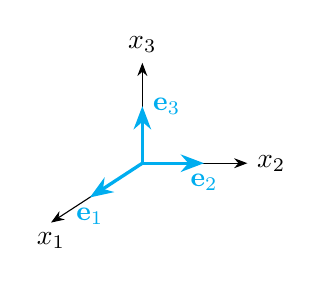
\begin{tikzpicture}[>=Stealth,scale=0.58]
  \draw[->] (0,0)--(-2,-1.3) node[below] {$x_1$};
  \draw[->] (0,0)--(2.3,0) node[right] {$x_2$};
  \draw[->] (0,0)--(0,2.2) node[above] {$x_3$};
  \draw[->,very thick,cyan] (0,0)--(-1.15,-.75) node[below] {$\vect e_1$};
  \draw[->,very thick,cyan] (0,0)--(1.35,0) node[below] {$\vect e_2$};
  \draw[->,very thick,cyan] (0,0)--(0,1.25) node[right] {$\vect e_3$};
\end{tikzpicture}

The standard basis for $\R^3$.
\end{center}
\end{frame}

% Source slide 40
\begin{frame}[shrink=15]{THE SPANNING SET THEOREM}
\begin{itemize}
\item \textbf{Theorem 5:} Let $S=\{\vect v_1,\ldots,\vect v_p\}$ be a set in $V$, and let $H=\Span\{\vect v_1,\ldots,\vect v_p\}$.
\begin{enumerate}
\item[(a.)] If one of the vectors in $S$---say, $\vect v_k$---is a linear combination of the remaining vectors in $S$, then the set formed from $S$ by removing $\vect v_k$ still spans $H$.
\item[(b.)] If $H\ne\{0\}$, some subset of $S$ is a basis for $H$.
\end{enumerate}
\item \textbf{Proof:}
\begin{enumerate}
\item[(a.)] By rearranging the list of vectors in $S$, if necessary, we may suppose that $\vect v_p$ is a linear combination of $\vect v_1,\ldots,\vect v_{p-1}$---say,
\end{enumerate}
\end{itemize}
\end{frame}

% Source slide 41
\begin{frame}[shrink=16]{THE SPANNING SET THEOREM}
\[
\vect v_p=a_1\vect v_1+\cdots+a_{p-1}\vect v_{p-1} \tag{3}
\]
\begin{itemize}
\item Given any $\vect x$ in $H$, we may write
\[
\vect x=c_1\vect v_1+\cdots+c_{p-1}\vect v_{p-1}+c_p\vect v_p \tag{4}
\]
for suitable scalars $c_1,\ldots,c_p$.
\item Substituting the expression for $\vect v_p$ from (3) into (4), it is easy to see that $\vect x$ is a linear combination of $\vect v_1,\ldots,\vect v_{p-1}$.
\item Thus $\{\vect v_1,\ldots,\vect v_{p-1}\}$ spans $H$, because $\vect x$ was an arbitrary element of $H$.
\end{itemize}
\end{frame}

% Source slide 42
\begin{frame}[shrink=13]{THE SPANNING SET THEOREM}
\begin{enumerate}
\item[(b.)] If the original spanning set $S$ is linearly independent, then it is already a basis for $H$.
\begin{itemize}
\item Otherwise, one of the vectors in $S$ depends on the others and can be deleted, by part (a).
\item So long as there are two or more vectors in the spanning set, we can repeat this process until the spanning set is linearly independent and hence is a basis for $H$.
\item If the spanning set is eventually reduced to one vector, that vector will be nonzero (and hence linearly independent) because $H\ne\{0\}$.
\end{itemize}
\end{enumerate}
\end{frame}

% Source slide 43
\begin{frame}[shrink=15]{THE SPANNING SET THEOREM}
\begin{itemize}
\item \textbf{Example 7:} Let
\[
\vect v_1=\begin{bmatrix}0\\2\\-1\end{bmatrix},
\qquad
\vect v_2=\begin{bmatrix}2\\2\\0\end{bmatrix},
\qquad
\vect v_3=\begin{bmatrix}6\\16\\-5\end{bmatrix},
\]
and $H=\Span\{\vect v_1,\vect v_2,\vect v_3\}$. Note that $\vect v_3=5\vect v_1+3\vect v_2$, and show that $\Span\{\vect v_1,\vect v_2,\vect v_3\}=\Span\{\vect v_1,\vect v_2\}$. Then find a basis for the subspace $H$.
\item \textbf{Solution:} Every vector in $\Span\{\vect v_1,\vect v_2\}$ belongs to $H$ because
\[
c_1\vect v_1+c_2\vect v_2=c_1\vect v_1+c_2\vect v_2+0\vect v_3.
\]
\end{itemize}
\end{frame}

% Source slide 44
\begin{frame}[shrink=14]{THE SPANNING SET THEOREM}
\begin{itemize}
\item Now let $\vect x$ be any vector in $H$---say,
\[
\vect x=c_1\vect v_1+c_2\vect v_2+c_3\vect v_3.
\]
\item Since $\vect v_3=5\vect v_1+3\vect v_2$, we may substitute
\begin{align*}
\vect x&=c_1\vect v_1+c_2\vect v_2+c_3(5\vect v_1+3\vect v_2)\\
&=(c_1+5c_3)\vect v_1+(c_2+3c_3)\vect v_2.
\end{align*}
\item Thus $\vect x$ is in $\Span\{\vect v_1,\vect v_2\}$, so every vector in $H$ already belongs to $\Span\{\vect v_1,\vect v_2\}$.
\item We conclude that $H$ and $\Span\{\vect v_1,\vect v_2\}$ are actually the set of vectors.
\item It follows that $\{\vect v_1,\vect v_2\}$ is a basis of $H$ since $\{\vect v_1,\vect v_2\}$ is linearly independent.
\end{itemize}
\end{frame}

% Source slide 45
\begin{frame}[shrink=15]{BASIS FOR $\Col B$}
\begin{itemize}
\item \textbf{Example 8:} Find a basis for $\Col B$, where
\[
B=[\vect b_1\ \vect b_2\ \cdots\ \vect b_5]
=\begin{bmatrix}
1&4&0&2&0\\
0&0&1&-1&0\\
0&0&0&0&1\\
0&0&0&0&0
\end{bmatrix}.
\]
\item \textbf{Solution:} Each nonpivot column of $B$ is a linear combination of the pivot columns.
\item In fact, $\vect b_2=4\vect b_1$ and $\vect b_4=2\vect b_1-\vect b_3$.
\item By the Spanning Set Theorem, we may discard $\vect b_2$ and $\vect b_4$, and $\{\vect b_1,\vect b_3,\vect b_5\}$ will still span $\Col B$.
\end{itemize}
\end{frame}

% Source slide 46
\begin{frame}[shrink=14]{BASIS FOR $\Col B$}
\begin{itemize}
\item Let
\[
S=\{\vect b_1,\vect b_3,\vect b_5\}
=\left\{
\begin{bmatrix}1\\0\\0\\0\end{bmatrix},
\begin{bmatrix}0\\1\\0\\0\end{bmatrix},
\begin{bmatrix}0\\0\\1\\0\end{bmatrix}
\right\}.
\]
\item Since $\vect b_1\ne0$ and no vector in $S$ is a linear combination of the vectors that precede it, $S$ is linearly independent. (Theorem 4).
\item Thus $S$ is a basis for $\Col B$.
\end{itemize}
\end{frame}

% Source slide 47
\begin{frame}[shrink=14]{BASES FOR $\Nul A$ AND $\Col A$}
\begin{itemize}
\item \sourcehead{Theorem 6:} The pivot columns of a matrix $A$ form a basis for $\Col A$.
\item \textbf{Proof:} Let $B$ be the reduced echelon form of $A$.
\item The set of pivot columns of $B$ is linearly independent, for no vector in the set is a linear combination of the vectors that precede it.
\item Since $A$ is row equivalent to $B$, the pivot columns of $A$ are linearly independent as well, because any linear dependence relation among the columns of $A$ corresponds to a linear dependence relation among the columns of $B$.
\end{itemize}
\end{frame}

% Source slide 48
\begin{frame}[shrink=13]{BASES FOR $\Nul A$ AND $\Col A$}
\begin{itemize}
\item For this reason, every nonpivot column of $A$ is a linear combination of the pivot columns of $A$.
\item Thus the nonpivot columns of a may be discarded from the spanning set for $\Col A$, by the Spanning Set Theorem.
\item This leaves the pivot columns of $A$ as a basis for $\Col A$.
\item \textbf{Warning:} The pivot columns of a matrix $A$ are evident when $A$ has been reduced only to echelon form.
\item But, be careful to use the pivot columns of $A$ itself for the basis of $\Col A$.
\end{itemize}
\end{frame}

% Source slide 49
\begin{frame}[shrink=12]{BASES FOR $\Nul A$ AND $\Col A$}
\begin{itemize}
\item Row operations can change the column space of a matrix.
\item The columns of an echelon form $B$ of $A$ are often not in the column space of $A$.
\item \textbf{Two Views of a Basis}
\item When the Spanning Set Theorem is used, the deletion of vectors from a spanning set must stop when the set becomes linearly independent.
\item If an additional vector is deleted, it will not be a linear combination of the remaining vectors, and hence the smaller set will no longer span $V$.
\end{itemize}
\end{frame}

% Source slide 50
\begin{frame}{TWO VIEWS OF A BASIS}
\begin{itemize}
\item Thus a basis is a spanning set that is as small as possible.
\item A basis is also a linearly independent set that is as large as possible.
\item If $S$ is a basis for $V$, and if $S$ is enlarged by one vector---say, $\vect w$---from $V$, then the new set cannot be linearly independent, because $S$ spans $V$, and $\vect w$ is therefore a linear combination of the elements in $S$.
\end{itemize}
\end{frame}

\end{document}
